\documentclass{article}
\usepackage[utf8]{inputenc}
\usepackage{hyperref}
\usepackage{graphicx}
\setlength{\parskip}{1em}
\usepackage[margin=1.0in]{geometry}
\usepackage{pgfplots}
\usepackage{subfig}
\pgfplotsset{width=10cm,compat=1.9}
\usepgfplotslibrary{external}
\tikzexternalize

\title{Lab 3: Get the Net!\\
  \large ECSE 421: Embedded Systems \\ Department of Electrical and Computer Engineering \\ McGill University \\ Version 1.0}
\author{Adam Cavatassi and Jeremy Cooperstock}
\date{Winter 2018}

\begin{document}

\maketitle

\section{Introduction}
In this lab, you will learn the basics of a neural network inference engine. You have been provided the weights and parameters for a pre-trained neural network that will allow your myRIO board to detect one of three spatial orientations in real-time. These instructions will guide you through the basics of a neural network, the best method to import the network weights into your project, and outline the expectations for your submission. All setup and lab instructions have been verified to work with LabVIEW 2016 on the PCs in Trottier Building Room 5090. 

\section{Neural network preliminaries}

The rest of the labs in this course as well as your final project will involve neural networks. These are trained to make predictions by being presented with examples from a labeled training set, consisting of a set of inputs, or features, and the corresponding output, over a (typically large) number of iterations.
Neural networks are loosely inspired by models of biological neurons. An example of such an artificial neuron, depicted in Fig.~\ref{fig:perceptron}, calculates the dot product of an input vector, $\mathbf{x}$ of dimension $N$, with a weight vector, $\mathbf{w}$ as

\begin{equation}
    \alpha = \sum\limits_{i=0}^{N-1} w_i x_i + b
\end{equation}

where $b$ is an optional bias offset. 

\begin{figure}[h]
\centering
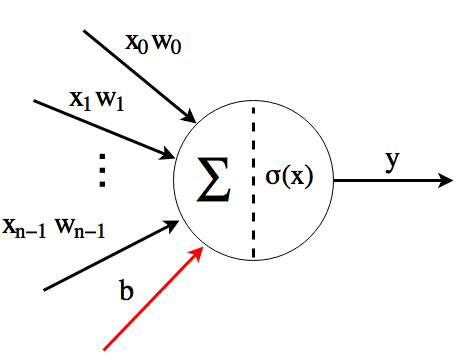
\includegraphics[scale=0.6]{figs/perceptron.png}
\caption{A single artificial neuron.}
\label{fig:perceptron}
\end{figure}

In essence, Equation (1) determines on which side of a decision boundary, defined by the weights, the input vector lies.  Such a neuron can thus be used as a linear classifier.  
The calculated value, $\alpha$ may then be passed through an activation function, $\Sigma$.  
For the original perceptron algorithm from 1957, this activation function is the simple step function. 
Other activation functions, such as the sigmoid, $\sigma(\alpha)$ and hyperbolic tangent function, $\tanh(\alpha)$, are often used, and for deep learning, a popular function is the \textbf{re}ctified \textbf{l}inear \textbf{u}nit, or \textit{reLU}, which calculates $\mathrm{reLU}(\alpha) = max(0, \alpha)$.
These activation functions are illustrated in Fig.~\ref{fig:plots}. 

The activation function serves to emulate the action potential of a biological neuron. When a specific range of input values are applied, the neuron will "fire" to indicate a correlation has been detected. This functionality is facilitated by the non-linearity.

\begin{figure}[h!]
\centering
\begin{tikzpicture}
\begin{axis}[
    axis lines = left,
    xlabel = $\alpha$,
    ylabel = {$act(\alpha)$},
    legend pos = outer north east
]
%Below the red parabola is defined
\addplot [
    domain=-3:3, 
    samples=100, 
    color=red,
]
{max(0, x)};
\addlegendentry{$reLU(\alpha)$}
%Here the blue parabloa is defined
\addplot [
    domain=-3:3, 
    samples=100, 
    color=blue,
    ]
    {1/(1+exp(-x))};
\addlegendentry{$\sigma(\alpha)$}

\addplot [
    domain=-3:3, 
    samples=100, 
    color=green,
    ]
    {tanh(x)};
\addlegendentry{$tanh(\alpha)$}
 
\end{axis}
\end{tikzpicture}
\caption{Plots of useful activation functions.}
\label{fig:plots}
\end{figure}

A single neuron can only classify a set of inputs into one of two classes.  To gain more decision power, multiple neurons or \textit{nodes} may be combined together in layers to form a multi-layer network, which allows for detection of multiple combinations of features.  Nodes in subsequent layers use as inputs the activation values of nodes from previous layers. The number of layers in a network is a tunable hyper-parameter, as is the number of nodes in any given layer. The large number of these hyper-parameters can make neural networks difficult to optimize.

A neural network always has an \textit{input layer} and an \textit{output layer}. The input layer consists of a number of nodes equal to the number of input features in the data.  These nodes are not artificial neurons, but rather, represent the input values, directly.  The number of nodes in the output layer should be equal to the number of classes the network is trying to classify. 
A network will typically also have one or more \textit{hidden layers} to enable further decision-making power when working with complex data sets. 
A two-dimensional weight matrix represents the connections between nodes in successive layers. One full iteration of applying inputs to the first layer and receiving a prediction at the output layer is called a \textit{forward pass}. The weights for the neural network can be learned using the \textit{back-propagation} algorithm, which will be covered in the next lab. 

Each output node is used to make a binary decision as to whether the input vector belongs to the corresponding class. As such, the output should be one-hot encoded, as seen in Table \ref{table:ohe}, for which the floating point values represent soft likelihoods that each of the classes is detected. In order to make a hard decision as to which class is being predicted, we simply take the output node with the highest value. 

\section{Orientation detection}

The training set for this lab was generated using a myRIO board. Each training example has five inputs and one output. The inputs, $\mathbf{x}$ each consist of a single sample of the acceleration data in the \textit{x}, \textit{y}, and \textit{z} axes, as well as the roll and pitch of the board. You will recall that you needed to collect the same data in your previous lab. The output, $o_i \in \{1,2,3\}$ for each example is an integer, representing one of the three possible orientations that the network is trained to recognize, as seen by the illumination of the corresponding LEDs in Fig.~\ref{fig:pos}.

\begin{figure}[h]
\centering
\hspace{-0cm}  
%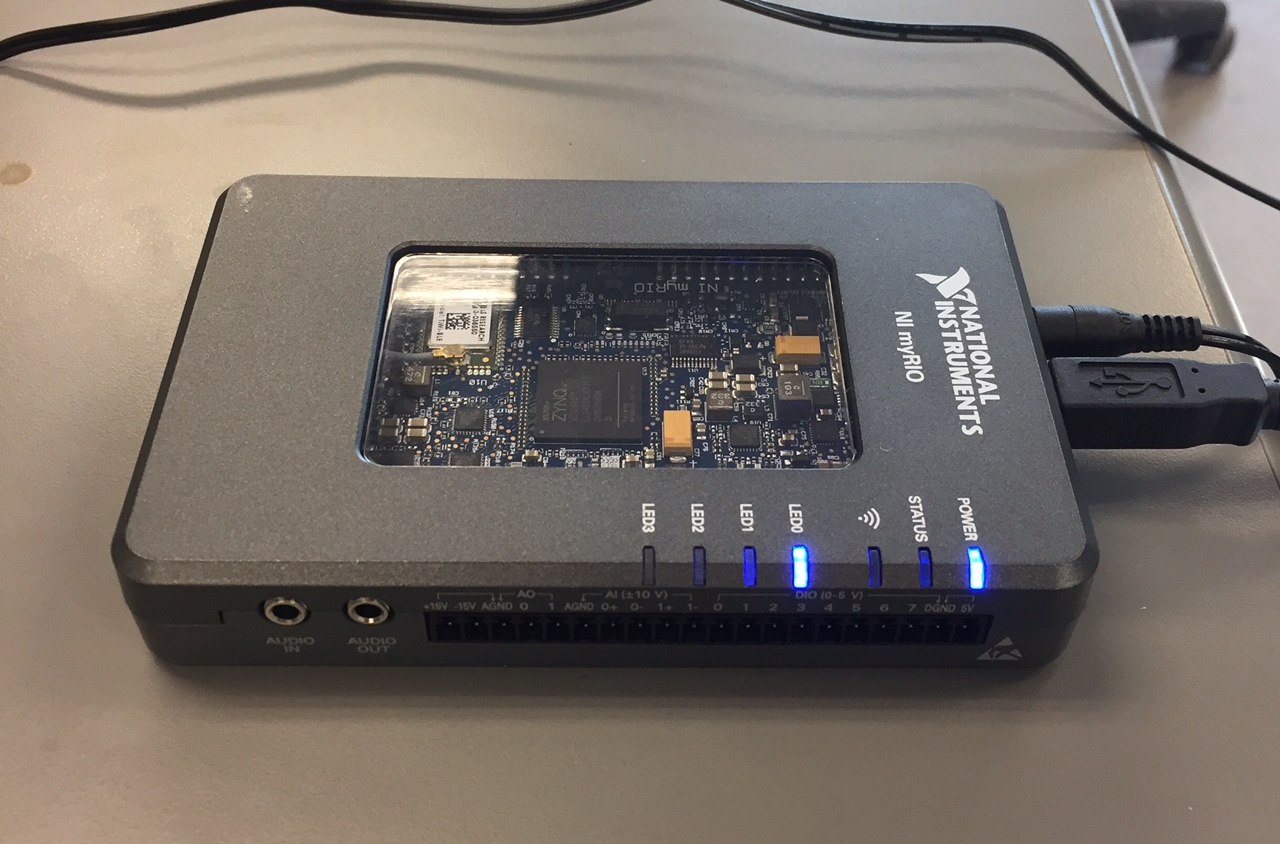
\includegraphics[scale=0.2]{figs/pos0.png}
%\caption{Position 0, LED0 is illuminated.}
%\label{fig:pos0}

\subfloat[Orientation 0]{{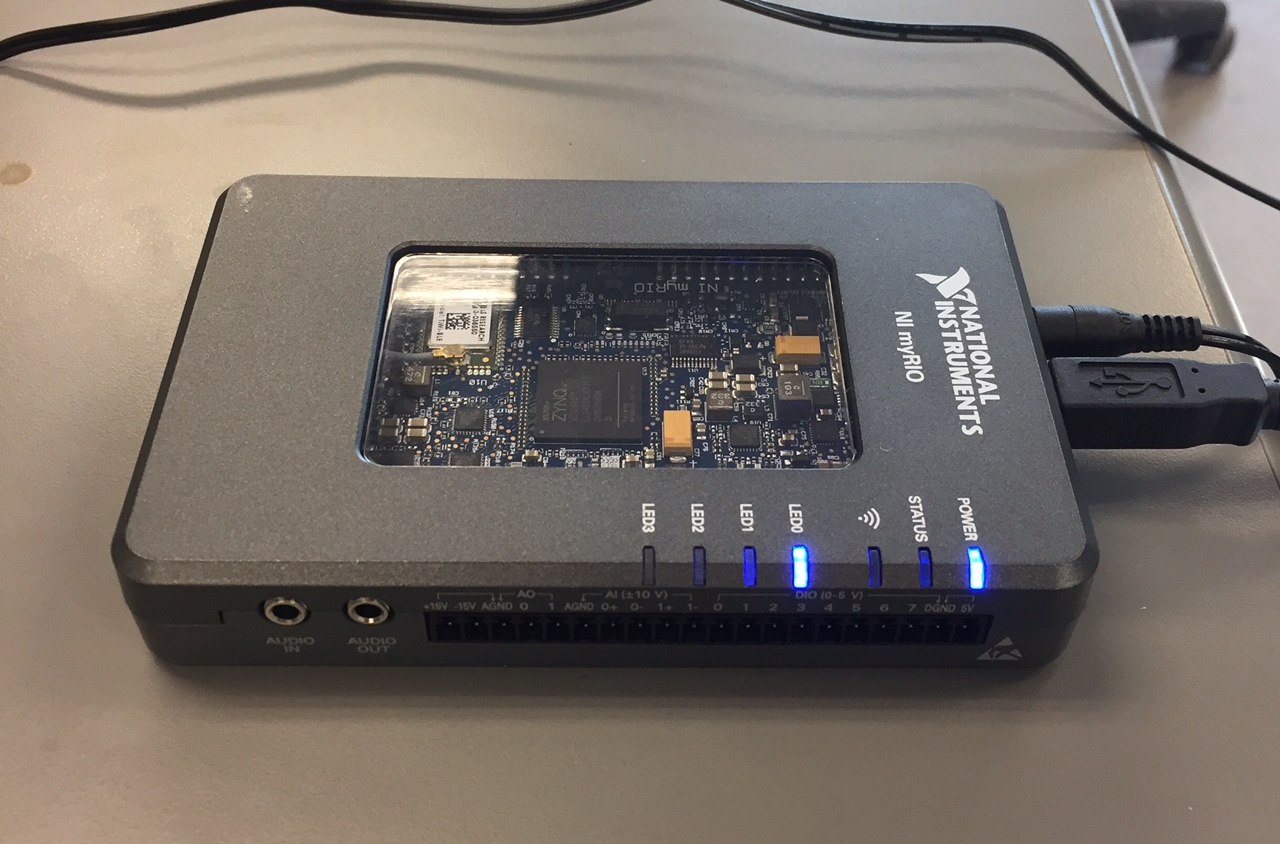
\includegraphics[width=.3\columnwidth]{figs/pos0.png} }}%
    %\qquad
\subfloat[Orientation 1]{{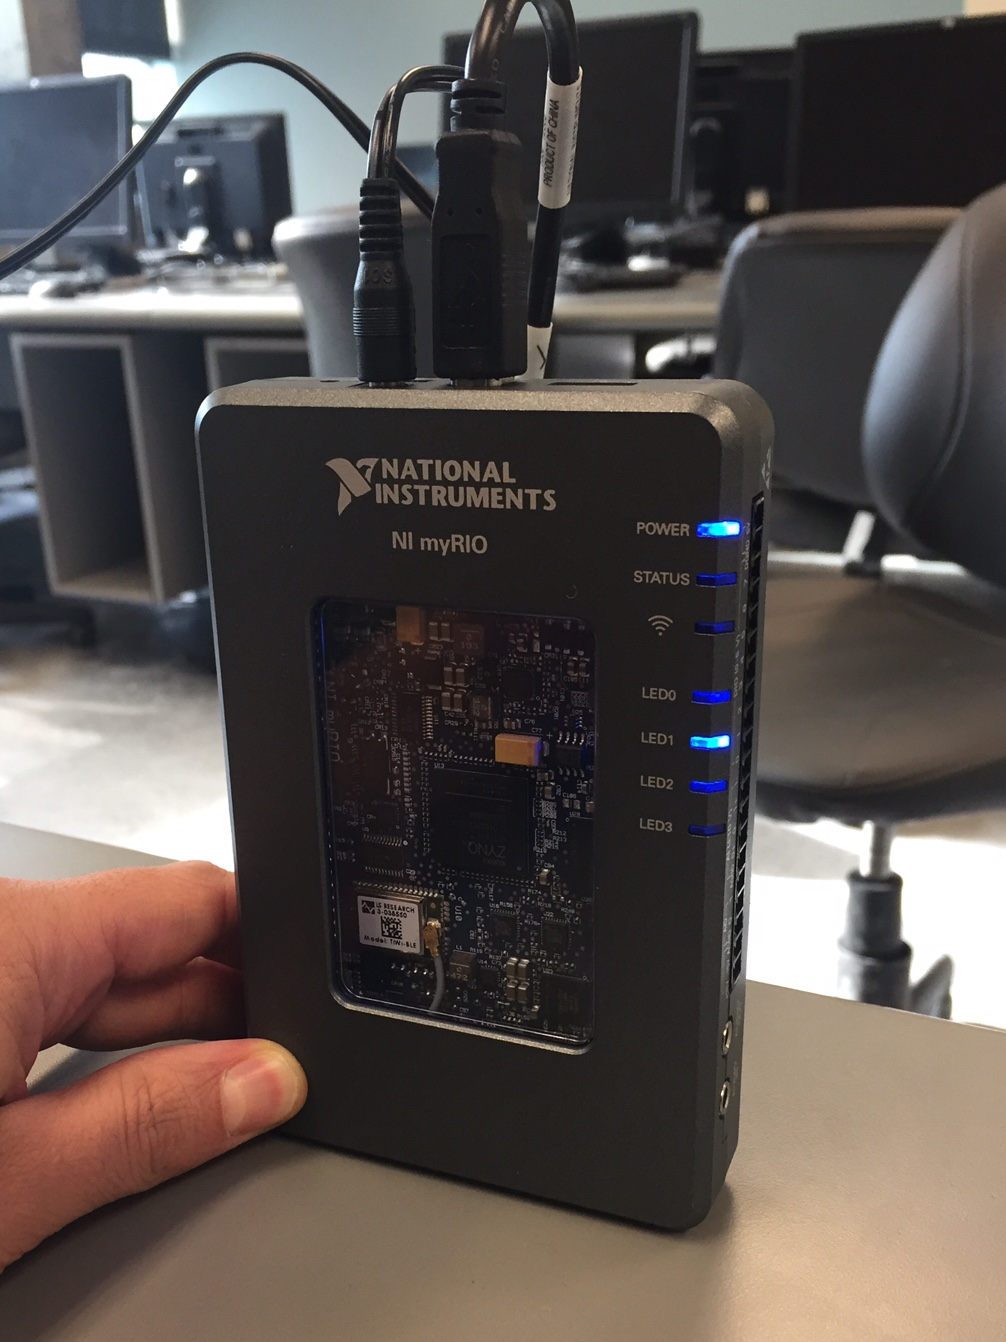
\includegraphics[width=.3\columnwidth]{figs/pos1.png} }}%
    %\qquad
\subfloat[Orientation 2]{{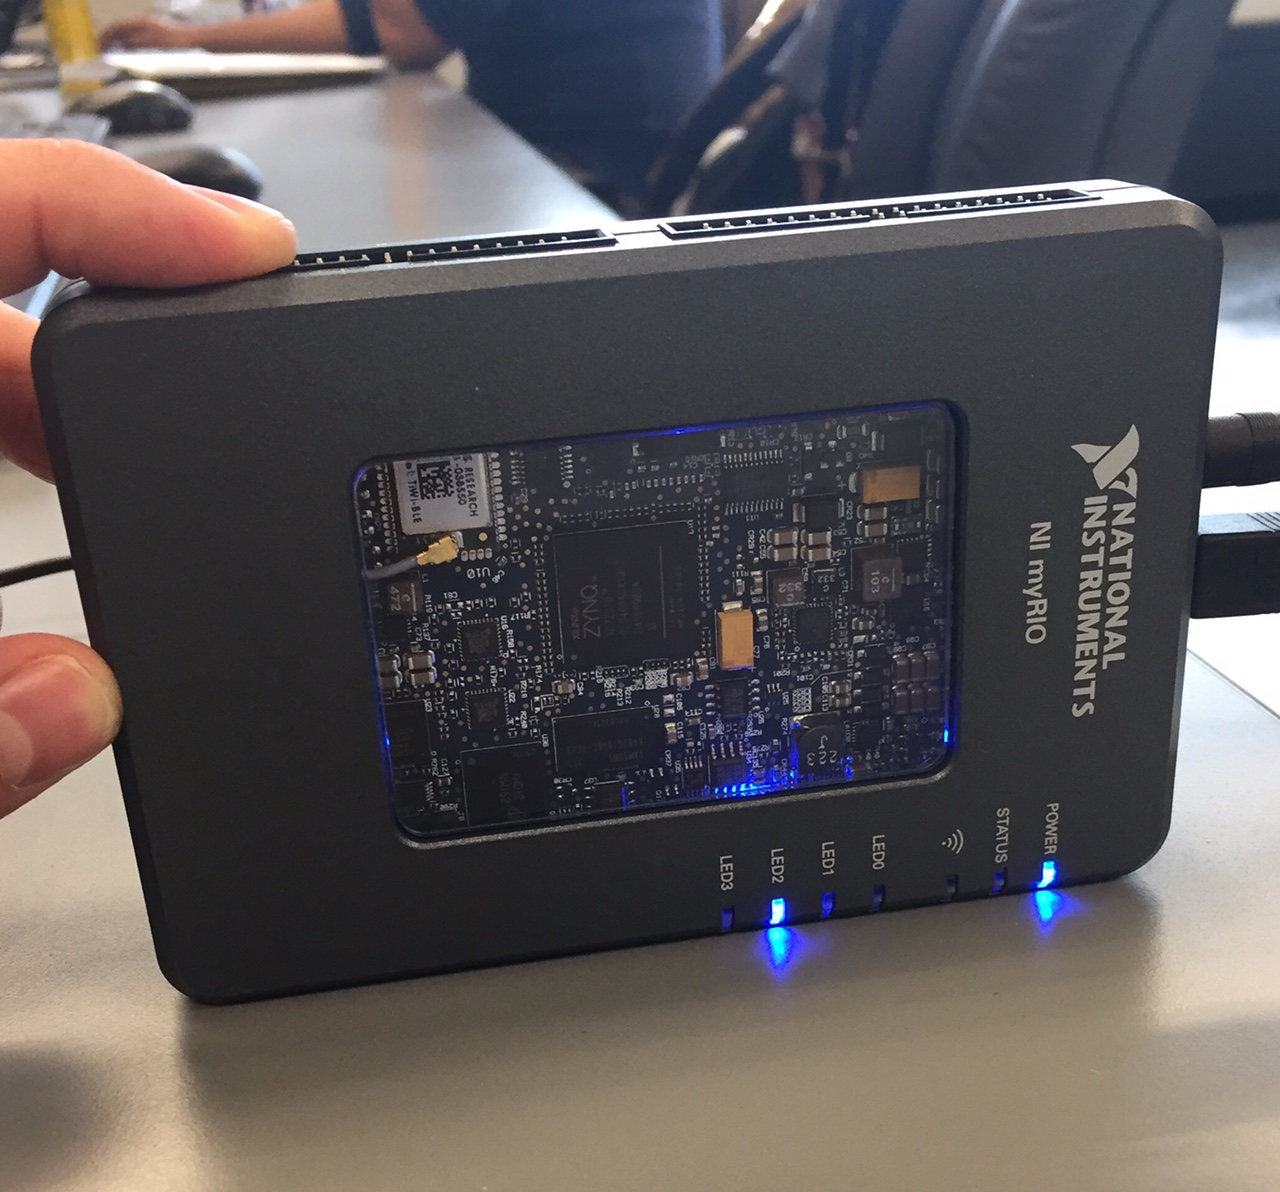
\includegraphics[width=.3\columnwidth]{figs/pos2.png} }}%
\caption{The three orientations of the myRIO board, with the corresponding LED illuminated.}
    
    
% 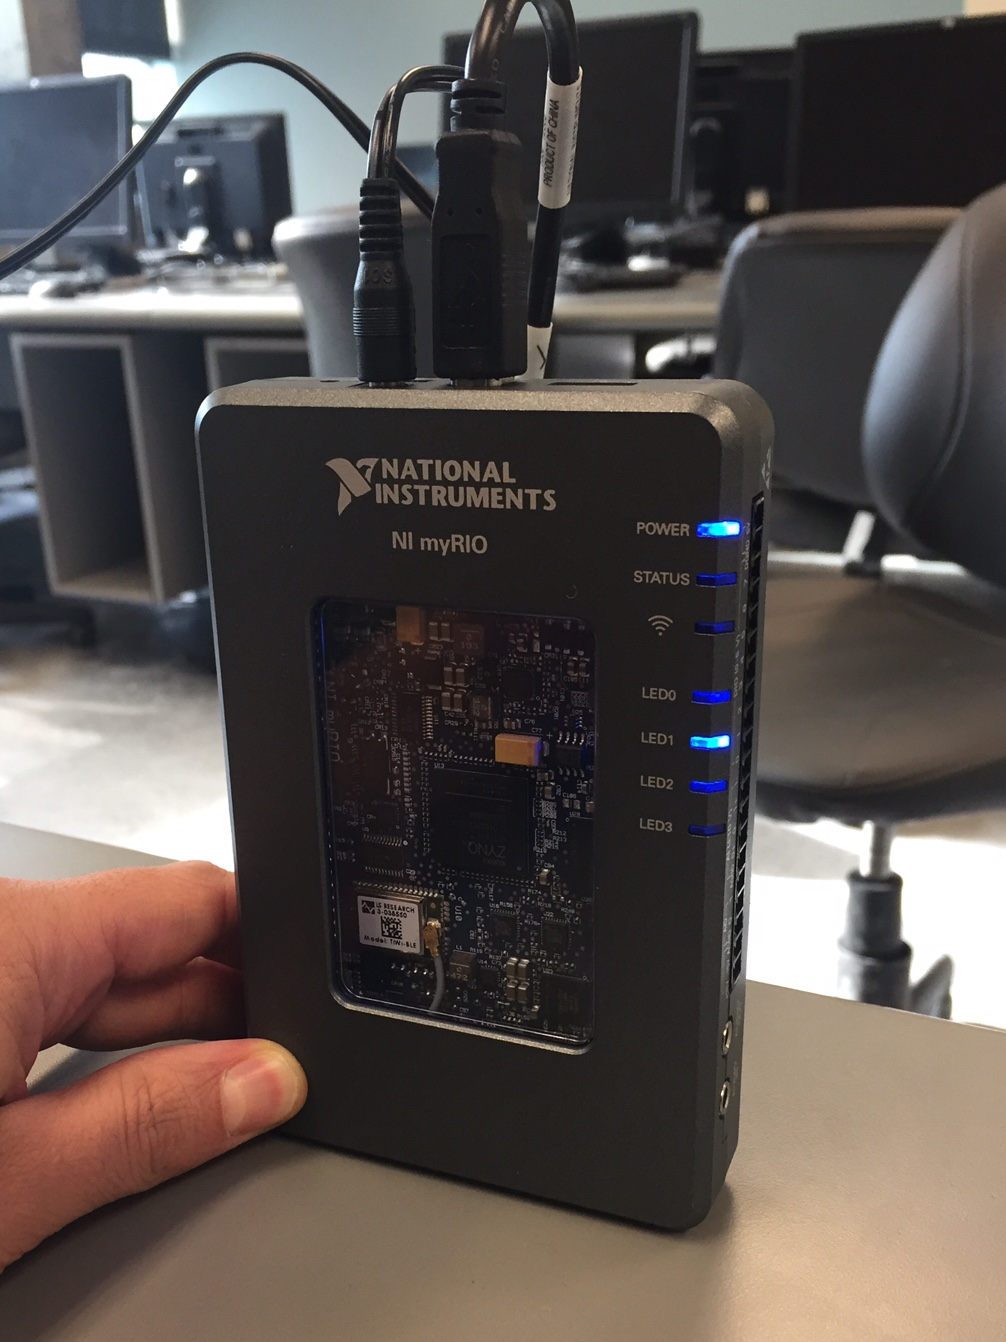
\includegraphics[scale=0.1]{figs/pos1.png}
% \caption{Position 1, LED1 is illuminated.}
% \label{fig:pos1}

% 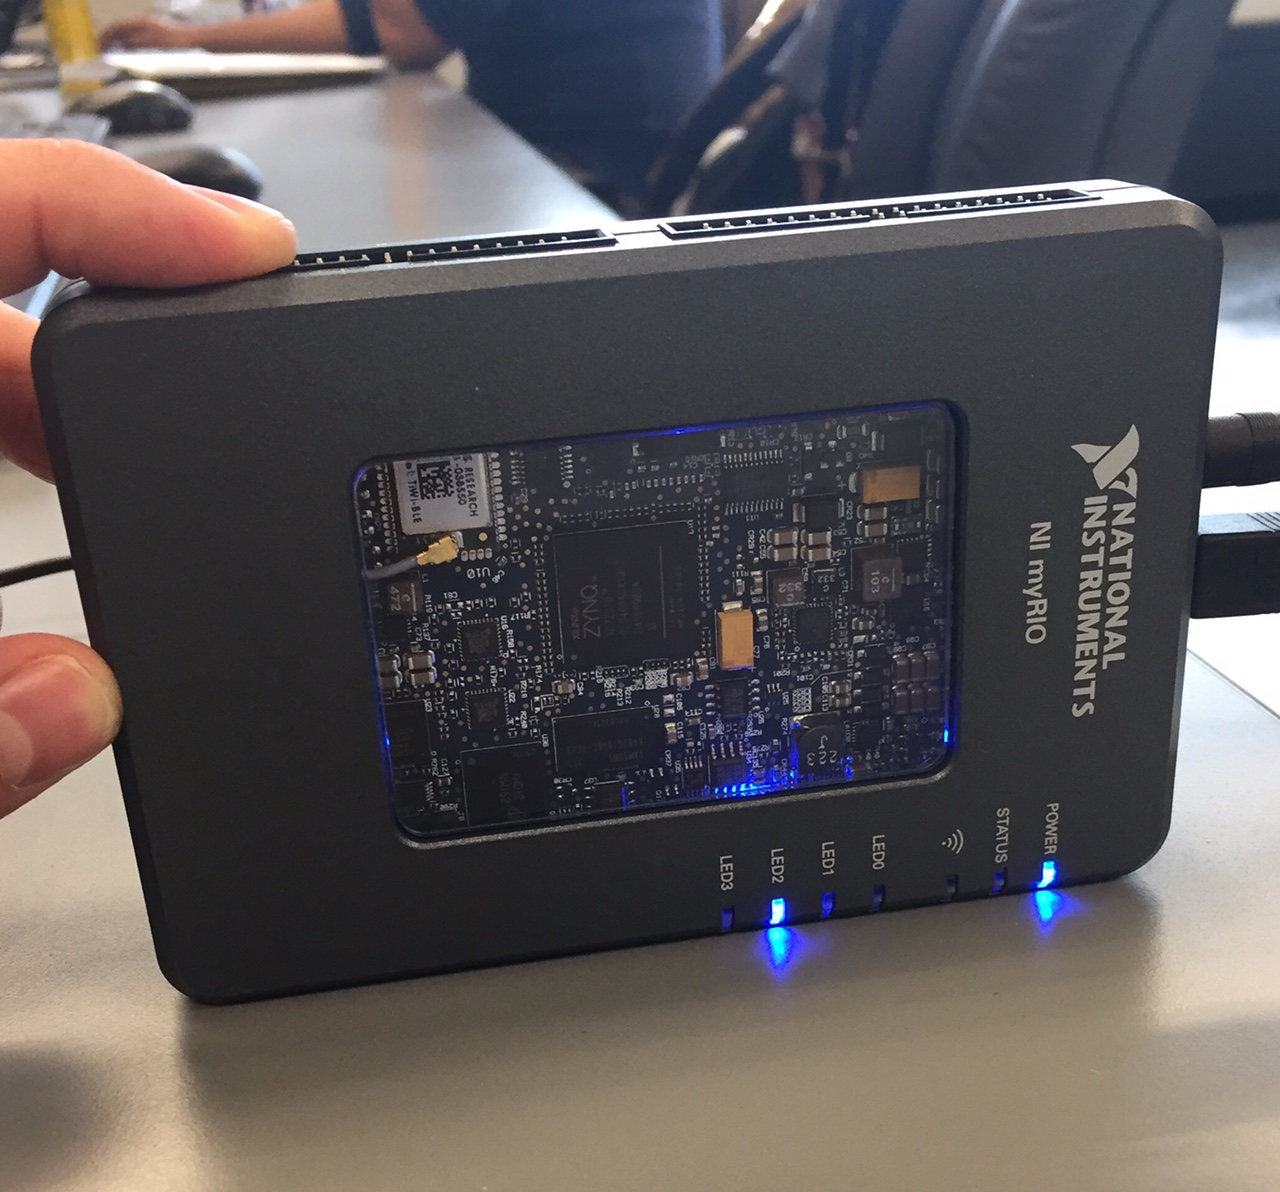
\includegraphics[scale=0.1]{figs/pos2.png}
% \caption{Position 2, LED2 is illuminated.}
\label{fig:pos}
\end{figure}

\subsection{Position-Net}

The neural network for this lab, cleverly named \textit{Position-Net}, has been pre-trained for you so you only have to implement the forward pass to create an inference engine. Position-Net consists of five input nodes, a single hidden layer with eight nodes, and an output layer of three nodes. The input nodes correspond to the five data values we know how to acquire: acceleration in the $x$, $y$, and $z$ axes, as well as the roll and pitch of the myRIO board. The input vector $[i_0, i_1, i_2, i_3, i_4]$ is equal to the signal vector $[a_x, a_y, a_z, \theta_{roll}, \theta_{pitch}]$. The three output nodes represent the output vector $[o_0, o_1, o_2]$. This vector corresponds to the three positions that the networks has been trained to recognize, as trained using the one-hot encoding method. The network will take a guess at which of the three positions the board is in based on the data supplied to the input nodes. For example, if the input vector $[0.001, -0.032, 0.998, 0.21, -0.018]$ were to be entered into Position-Net, you might get an output vector similar to $[0.923, 0.342, 0.098]$. In this case, the network thinks that position 0 is most likely, since $o_0$ has the highest value.  This network has 3 layers, so there are 2 weight matrices.  The activation function used in this neural network is the sigmoid function, as defined by Equation \ref{eq:sig}. A visual representation of Position-Net can be seen in Fig.~\ref{fig:position_net}.

\begin{figure}[h!]
\centering
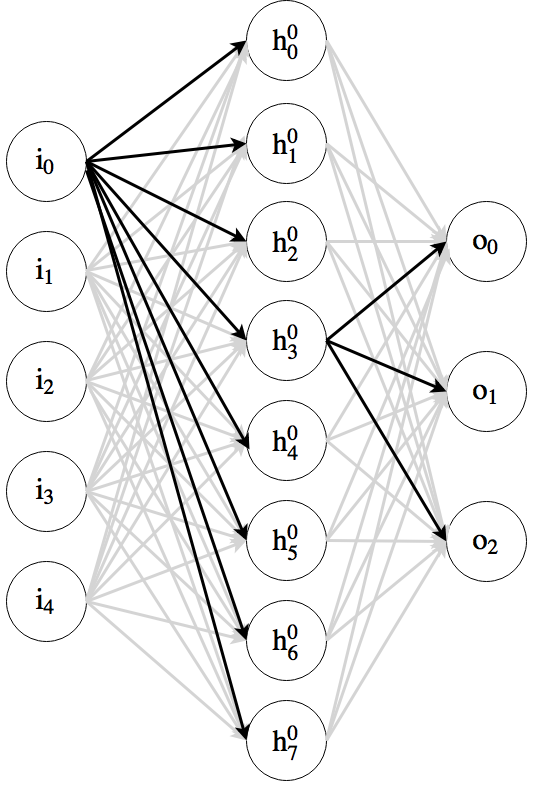
\includegraphics[scale=0.3]{figs/position_net.png}
\caption{Position-Net, consisting of 5 input nodes, 8 hidden nodes, and 3 output nodes.}
\label{fig:position_net}
\end{figure}

\begin{table}[h!]
\begin{center}
\begin{tabular}{ c c c }
 Position \# & One-hot encoding \\ 
 \hline
 0 & 100 \\ 
 1 & 010 \\  
 2 & 001
\end{tabular}
\caption{One-hot encoding for 3 positions.}
\label{table:ohe}
\end{center}
\end{table}

\begin{figure}[h!]
\centering
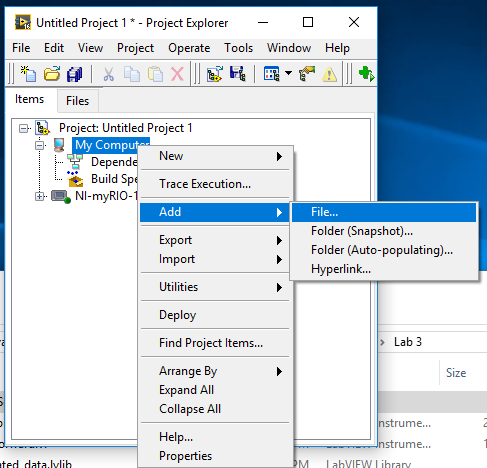
\includegraphics[scale=0.7]{figs/_1.png}
\caption{Add files to the PC target.}
\label{fig:_1}
\end{figure}

\begin{figure}[h!]
\centering
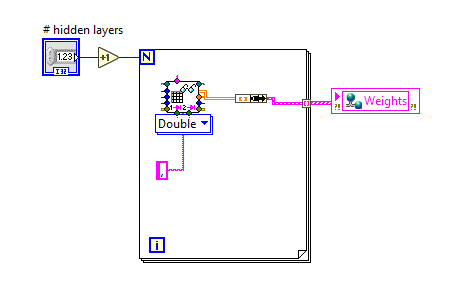
\includegraphics[scale=0.8]{figs/_3.png}
\caption{The VI used to import weight data from .csv files to shared variables.}
\label{fig:_3}
\end{figure}

\begin{figure}[h!]
\centering
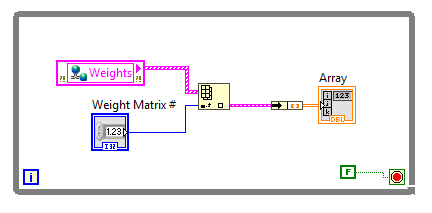
\includegraphics[scale=0.8]{figs/_7.png}
\caption{Build this VI to ensure the weight data is imported properly.}
\label{fig:_7}
\end{figure}

\begin{figure}[h!]
\centering
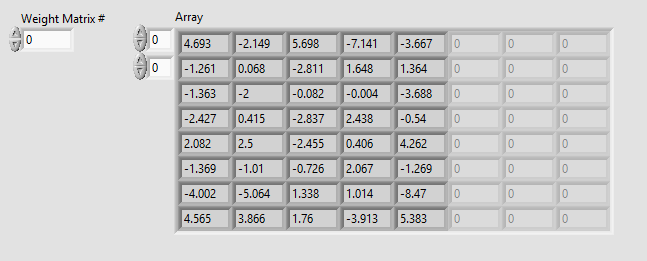
\includegraphics[scale=0.7]{figs/_8.png}
\caption{Ensure that the weights between the input layer and hidden layer are visible.}
\label{fig:_8}
\end{figure}

\begin{figure}[h!]
\centering
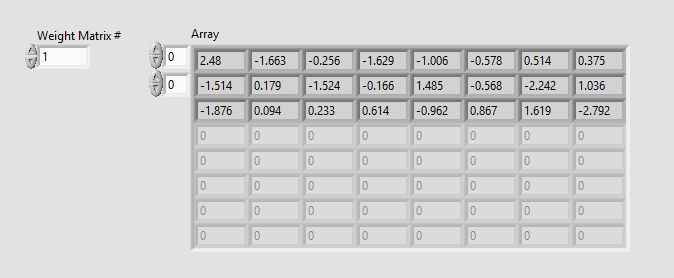
\includegraphics[scale=0.7]{figs/_9.png}
\caption{Ensure that the weights between the hidden layer and output layer are visible.}
\label{fig:_9}
\end{figure}

\begin{figure}[h!]
\centering
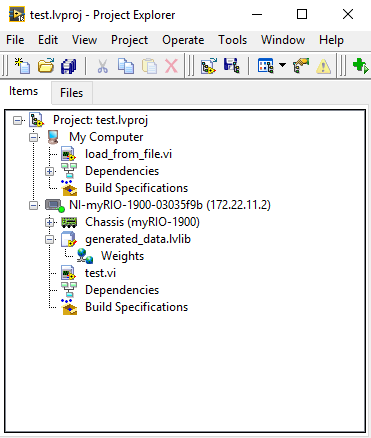
\includegraphics[scale=0.7]{figs/_A.png}
\caption{Your project explorer should look like this after adding all of the supplied files.}
\label{fig:_A}
\end{figure}

\subsection{Importing the network weights into your project}

To begin building Position-Net, download the .zip file called \textbf{ecse\_421\_lab\_3\_files}. Once extracted, the directory contains the LabVIEW library file \textbf{generated\_data.lvlib}, the VI \textbf{load\_from\_file.vi}, and two 2D weight matrices stored as .csv files. The weights can be viewed in Excel. The weights connecting the input layer and the hidden layer are stored in \textbf{weights\_input\_h0.csv}, and the weights connecting the hidden layer and the output layer are found in \textbf{weights\_h0\_out.csv}. 

Just as with the previous lab, start a new project in LabVIEW with your myRIO board as a target. You will need to add the library file to your project, as outlined in Fig. \ref{fig:_1}. Right-click \textbf{My Computer}, and add the library file and the VI. Drag the \textbf{generated\_data} library down to the myRIO target. The library will contain a shared variable called \textbf{Weights}. A shared variable is necessary to be able to load the weight data onto the myRIO board. The myRIO has its own file system which is separate from the PC on which you are working. Because of this, saving files on the myRIO board does not allow for saving data on the PC. 

At this point, your project should look the same as the one in Fig. \ref{fig:_A}. The VI used to load the weights from file should be located on the local PC target, and the library and shared variable should be located on the myRIO target. Once you have ensured that the project is properly assembled, you can run \textbf{load\_from\_file.vi}, seen in Fig. \ref{fig:_3}. The VI consists of a simple FOR loop to populate the shared variable. Make sure that the \textbf{# hidden nodes} parameter is set to 1. If the VI is broken and not running, it may because LabVIEW did not find the shared variable at the right time. This can be fixed by adding a new shared variable reference, which can be found in the block diagram module search. If you do add a new shared variable reference, be sure to select the \textbf{Weights} variable from the drop down menu and delete the old broken reference. Once the VI does run, you will be prompted with a file selection dialog. Be sure to select \textbf{weights\_input\_h0.csv} first, and \textbf{weights\_h0\_out.csv} second. If you complete this step incorrectly, you can always re-run the VI and select the files properly. Note that every time you launch LabVIEW to work on your lab, you will need to re-run this VI to load the weights into the shared variable. The shared variable will \textit{not} retain the stored values after you close LabVIEW.

Once you have successfully run the \textbf{load\_from\_file} VI, you should make a test VI on your myRIO board to verify that the values are indeed stored in the shared variable. Build a VI that looks like the one in Fig. \ref{fig:_7}. The format of the shared variable is a 1D array of clusters. Clusters are a LabVIEW container that can be custom-built. In this case, the format of the clusters is a 2D array of doubles. Note that you need to unbundle a cluster in order to access its contents. In summary: the shared variable \textbf{Weights} is a 1D array of clusters of 2D arrays of double. The reason the weights are not in a more straightforward 3D array is because LabVIEW does not support jagged arrays. For a neural network, each 2D array of weights between layers will usually have dimensions of different sizes. Once your test VI is working, you should be able to view the contents of the weight arrays, as shown in Figs. \ref{fig:_8} and \ref{fig:_9}. Verify the values of the arrays with the .csv files in Excel. Note that the first set of weights is an $8 \times 5$ matrix, and the second set of weights is a $3 \times 8$ matrix.  

Now that you can see that the weights are properly stored in the shared variable, you can use them to build your feed forward inference engine by implementing Position-Net. Although Position-Net is a relatively small and simple neural network, it is important to note that a highly reconfigurable design will be very useful for future labs and projects. Hand-wiring the network together without any looping or modular configuration will make your work in this lab not very useful for future work. 


\section{Submission requirements}

For this lab, you will be required to submit a .zip file containing your project file, all VI files that are part of your project, and screenshots of each the final block diagram and final front panel for all VIs. You will also be required to submit a URL to a private YouTube video with a maximum length of 120 seconds which demonstrates the full functionality of the inference engine in real-time. Show that your inputs are your 5 signals from the previous lab, and your outputs are LED0, LED1, and LED2 on the myRIO board. Show that each position is clearly recognized by the neural network, as indicated by the LEDs. 

\end{document}
